% Include required packages
\documentclass{mxl-design}
\usepackage{listings}
\usepackage{float}

%====== Title Page ======%
% Setup document
\title{Mercury2 Revised Design}
\author{Jimmy Blanchard}
\docnum{0.3.0}

% Start the document
\begin{document}
\maketitle

% Document revision history
\vspace{5in}
\begin{table}[H]
\begin{center}
\begin{tabular}{|p{0.5in}|p{1.2in}|p{2.8in}|p{0.5in}|}
	\hline
	\bf Rev & \bf Date & \bf Notes & \bf Authors \\ 
	\hline
	0.3.0 & December 2, 2012 & Mercury2 design revisions. & jimblanc \\ \hline
\end{tabular}
\end{center}
\end{table}

%====== Table of Contents ======%
\clearpage
\tableofcontents
\clearpage

%==========================%
%====== Introduction ======%
%==========================%
\section{Introduction}
Mercury2 is the next evolution of the Mercury Ground Station System. It will allow satellite operators to reserve, configure, and use ground station hardware while still giving ground station operators complete control over their hardware. Mercury2 will include a feature rich web interface to enable ground station control over the network by satellite and ground station operators alike.

%=== Terms ===%
\subsection{Terms and Definitions}
This section contains a list terms and acronyms commonly used in this document.

\begin{table}[h]
	\footnotesize {\begin{tabular}{ p{5cm} p{10cm} }
		\textbf{Mercury2} & Refers to the ground station management system as a whole, including all sub-components (e.g. the hardware manager and user interface).\\[.2cm]
		\textbf{Hardware Manager} & An application that runs on a computer that is physically attached to the ground station hardware. It is responsible for processing ground station commands (from the user interface) and facilitating data transfer.\\[.2cm]
		\textbf{User Interface} & This application runs on a web server and provides the interfaces to allow ground station and satellite operators to interact with and control the ground station. It relays commands from the user to the hardware manager.\\[.2cm]
		\textbf{Hardware Pipeline} & A collection of related hardware used to either transmit or receive information to and from the radio (or both, if the hardware supports it).\\[.2cm]
		\textbf{Ground Station} & Refers to the complete Mercury2 system (i.e. the user interface and any hardware managers associated with it). Generally, this means several computers and pieces of hardware on the same local area network.\\[.2cm]
		\textbf{Satellite} & A device in orbit that Mercury2 configured ground stations can connect to.\\[.2cm]
		\textbf{Pass} & A transit of a satellite over a ground station. Passes can be scheduled, which reserves a specific hardware pipeline for the duration of the pass. Scheduled passes are identified by the satellite name, orbit number, and ground station.\\[.2cm]
		\textbf{Timestamp} & The duration of scheduled command sessions for Mercury2 will be defined by a start and end timestamp. These timestamps will be simple UNIX timestamps indicating the start and end of the reservation.\\[.2cm]
		\textbf{Satellite Operator} & An entity that remotely reserves ground station use (via the user interface) and uses it to send and receive data from a satellite.\\[.2cm]
		\textbf{Ground Station Operator} & A user that is associated with the ground station and has some privileges over it (e.g. the ability to approve/reject reservation requests or the ability to configure hardware pipelines).\\[.2cm]
		\textbf{Ground Station Administrator} & The user with complete administrative control over the ground station.\\[.2cm]
		\textbf{MVC Framework} & Model-View-Controller framework. Refers to a common web application software design pattern.\\[.2cm]
		\textbf{YAML} & An easy-to-use configuration format. Will be used to configure the hardware manager.\\[.2cm]
		\textbf{Asynchronous} & A type of program design that allows tasks to be executed in an undefined order. This will be used in the hardware manager to allow it to respond to radio events.
	\end{tabular}}
	\caption{General Definitions}
	\label{tab:Mercury2 Definitions}
\end{table}

%=== Requirements ===%
\clearpage
\subsection{Application Requirements}
This section outlines the various requirements for the Mercury2 system. These are the requirements for the initial release of the application.

\subsubsection{User Interface Requirements}
The user interface component of Mercury2 will run on a net-accessible web server and will allow satellite and ground station operators to interact with the various configured hardware managers. Its primary features consist of the following items.

\begin{itemize}
	\item User authentication, authorization, and management
		\begin{itemize}
			\item Registration and account management
			\item API access key management
			\item User permissions
		\end{itemize}
	\item Ground station administration
		\begin{itemize}
			\item Hardware pipeline configuration
			\item Enable or disable ground station access
			\item View and modify pending ground station schedules
			\item Approve or deny reservation requests (if approval required)
			\item Manual override
		\end{itemize}
	\item Ground station reservation
		\begin{itemize}
			\item Reservation utility to allow satellite operators to reserve ground station pipeline use
			\item Current reservation schedule viewer
			\item Upcoming passes over the ground station
			\item Automatic TLE updates
		\end{itemize}
	\item Satellite tracking during pass
		\begin{itemize}
			\item retroTrack-esque tracker
			\item Various data streams from the hardware manager (connection permitting) such as a waterfall plot or web cam feed
			\item Telemetry stream connection settings (i.e. IP address, port, etc.)
		\end{itemize}
	\item SSL encryption and protection from various exploits	
	\item Complete access and error logs
\end{itemize} 

\subsubsection{Hardware Manager Requirements}
The hardware manager component of Mercury2 will run on a computer physically connected to the ground station hardware. It is responsible for parsing ground station commands from the user interface as well as providing the sockets that satellite operators will use to transmit and receive data to and from their satellite.

\begin{itemize}
	\item Run schedules and commands received from the user interface
	\item Asynchronously manage hardware and data streams
	\item Connect to hardware via drivers
	\item Buffer and record telemetry data
	\item Periodically sync schedules from the user interface	
	\item Provide sockets (defined by the schedule) to allow satellite operators to transmit commands to and receive telemetry from the ground station
	\item Key encrypted security for all data streams (using keys from the user interface)
\end{itemize}

%==================================%
%====== Architecture Details ======%
%==================================%
\clearpage
\section{Architecture Details}
This section will detail each component of the Mercury2 system displayed in figure 1 (below).

\begin{figure}[hbtp]
\centering
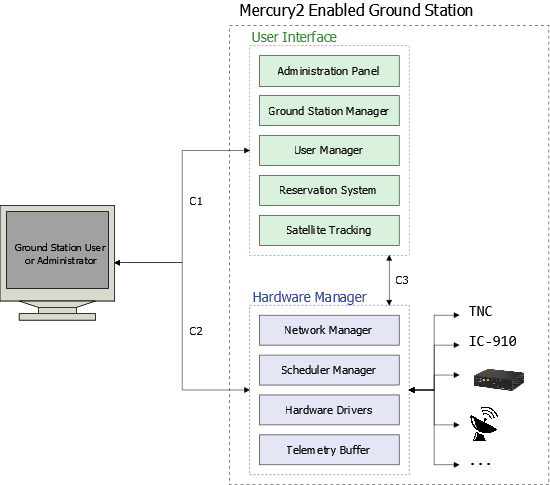
\includegraphics[scale=.55]{Architecture_Diagram.png}
\caption{Mercury2 Architecture Overview}
\end{figure}

%=== User Interface ===%
\subsection{User Interface}
The user interface for Mercury2 will consist of an application running on a web server that will allow satellite and ground station operators to interact with the ground station. This web application will be responsible for managing user permissions, maintaining the ground station reservation schedule, providing ground station feedback to satellite operators during reservations, and sending commands to the hardware manager. Each major component of the user interface (illustrated in figure 1) will be described in further detail in the following sections.

\paragraph{Platform Details}
The user interface application will be developed on top of a popular Python MVC web framework, known as \textit{Django}, running on an Apache web server. Django comes with many useful features right out of the box such as user management, user input sterilization, and a well developed templating system which will greatly reduce development time. The application will make use of a MySQL database to store user information, schedule details, and user activity logs, among other things.

\paragraph{Security}
Because the user interface has access to sensitive user information and direct control over the ground station, security and access control will be very important. Fortunately, Django comes with many useful security features by default such as user input sterilization, protection against cross-site scripting attacks, password hashing, and user permission management. User permissions will be configured to give users various levels of control over the ground station depending on their role (satellite operator, ground station operator, administrator, etc.). This mechanism will be detailed in the User Manager section (2.1.1). In addition, the security protocols used to protect the hardware manager data and command streams will be detailed in section 2.3.1.

\subsubsection{User Manager}

\subsubsection{Reservation System}

\subsubsection{Satellite Tracking}

\subsubsection{Ground Station Manager}

\subsubsection{Administration Panel}

%=== Hardware Manager ===%
\subsection{Hardware Manager}

\subsubsection{Network Manager}

\subsubsection{Schedule Manager}

\subsubsection{Hardware Drivers}

\subsubsection{Telemetry Buffer}

%=== Data Flow ===%
\subsection{Data Flow}

\subsubsection{Security}

% End the document
\end{document}
